% ===============================================================
%  جلسه سوم
% ===============================================================
\chapter{نتایج اصول کولموگروف، آزمایش برنولی و استقلال آماری}

\section{مرور مباحث جلسه قبل}

در جلسات گذشته با سه مفهوم پایه آشنا شدیم:
\begin{itemize}
\item \textbf{نظریه مجموعه‌ها:} مفهوم مجموعه، عضویت، ضرب دکارتی و عملگرهایی مانند متمم، اجتماع، اشتراک و تفاضل.
\item \textbf{فضای احتمال:} یک سه‌تایی مرتب $(\Omega,\F,\Prob)$ که در آن $\Omega$ فضای نمونه، $\F$ یک میدان سیگما (\lr{$\sigma$-field}) روی $\Omega$ و بیانگر فضای رخدادها، و $\Prob$ یک اندازه احتمال از $\F$ به بازه $[0,1]$ است.
\item \textbf{قوانین کولموگروف \lr{(Kolmogorov's Principles)}:} این قوانین به زبان ساده بیان می‌کنند که $\Prob$ یک اندازه (\lr{measure}) روی $\Omega$ است، با این شرط که $\Prob(\Omega)=1$.
\end{itemize}

\section{نتایج بدیهی قوانین کولموگروف}

تابع احتمال $\Prob$ صرفاً یک اندازه تعریف‌شده روی مجموعه $\Omega$ است، با این قید اضافی که $\Prob(\Omega)$ باید برابر ۱ شود. با استفاده از قضیه دمورگان و عملیات ساده روی مجموعه‌ها، می‌توان نتایج زیر را به دست آورد.

\begin{theorem}[احتمال متمم و تهی]
برای هر $A\in\F$:
\[\Prob(A^c)=1-\Prob(A),\qquad \Prob(\varnothing)=0.\]
\end{theorem}
\begin{proof}
$A$ و $A^c$ ناسازگارند و $A\cup A^c=\Omega$. پس طبق اصل جمع‌پذیری و نرمال بودن:
$1=\Prob(\Omega)=\Prob(A)+\Prob(A^c)$،
که نتیجه می‌دهد $\Prob(A^c)=1-\Prob(A)$. با قرار دادن $A=\Omega$ و توجه به $\Omega^c=\varnothing$ داریم $\Prob(\varnothing)=1-1=0$.
\end{proof}

\begin{theorem}[یکنوایی]
اگر $A\subseteq B$ آنگاه $\Prob(A)\le\Prob(B)$. به‌ویژه برای هر رویداد $0\le \Prob(A)\le 1$.
\end{theorem}
\begin{proof}
$B=A\cup(B\setminus A)$ و این دو مجموعه ناسازگارند. پس $\Prob(B)=\Prob(A)+\Prob(B\setminus A)\ge\Prob(A)$ زیرا $\Prob(B\setminus A)\ge0$.
\end{proof}

\begin{note}
\notetitle اصل اول کولموگروف، یعنی جمع‌پذیری احتمال تحت اجتماع شمارای مجموعه‌های ناسازگار، را پیش‌تر (جلسه قبل) به صورت شهودی و با تعریف «فرکانس نسبی رخدادها» برای احتمال نیز دیده بودیم.
\end{note}

\section{اصل شمول و عدم شمول \lr{(Inclusion--Exclusion Principle)}}

در جلسه قبل این اصل را در مورد اندازه (کاردینالیته) مجموعه‌ها دیده بودیم. همین اصل در مورد احتمال (یا هر اندازه یا \lr{measure} دیگری) نیز برقرار است.

\begin{theorem}[حالت دو و سه رویداد]
\[\Prob(A\cup B)=\Prob(A)+\Prob(B)-\Prob(A\cap B),\]
\[\Prob(A\cup B\cup C)=\Prob(A)+\Prob(B)+\Prob(C)-\Prob(A\cap B)-\Prob(A\cap C)-\Prob(B\cap C)+\Prob(A\cap B\cap C).\]
\end{theorem}
\begin{proof}
$A\cup B$ را به سه قطعه ناسازگار $A\setminus B$، $A\cap B$ و $B\setminus A$ افراز می‌کنیم. چون $\Prob(A)=\Prob(A\setminus B)+\Prob(A\cap B)$ و $\Prob(B)=\Prob(B\setminus A)+\Prob(A\cap B)$:
\[\Prob(A\cup B)=\Prob(A\setminus B)+\Prob(A\cap B)+\Prob(B\setminus A)=\Prob(A)+\Prob(B)-\Prob(A\cap B).\]
برای سه رویداد، رابطه دوتایی را برای $A\cup B$ و $C$ به کار می‌بریم:
$\Prob(A\cup B\cup C)=\Prob(A\cup B)+\Prob(C)-\Prob\big((A\cap C)\cup(B\cap C)\big)$
و با بسط دوباره دو جمله اول و آخر (و توجه به $(A\cap C)\cap(B\cap C)=A\cap B\cap C$) رابطه به دست می‌آید.
\end{proof}

\begin{figure}[H]
\centering
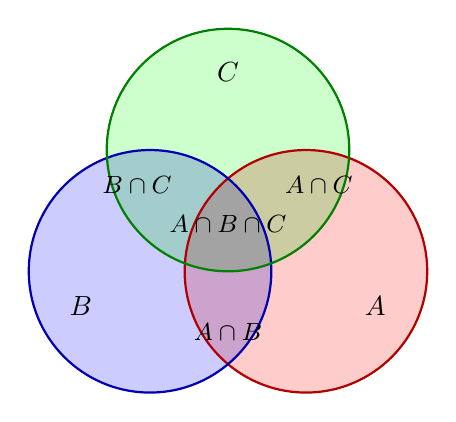
\begin{tikzpicture}[scale=1.1]
\begin{scope}[blend group=multiply]
\fill[red!20] (0.9,0) circle (1.4);
\fill[blue!20] (-0.9,0) circle (1.4);
\fill[green!20] (0,1.4) circle (1.4);
\end{scope}
\draw[red!70!black,thick] (0.9,0) circle (1.4);
\draw[blue!70!black,thick] (-0.9,0) circle (1.4);
\draw[green!50!black,thick] (0,1.4) circle (1.4);
\node at (1.7,-0.4) {$A$};
\node at (-1.7,-0.4) {$B$};
\node at (0,2.3) {$C$};
\node[font=\small] at (0,-0.7) {$A\cap B$};
\node[font=\small] at (0,0.55) {$A\cap B\cap C$};
\node[font=\small] at (1.05,1.0) {$A\cap C$};
\node[font=\small] at (-1.05,1.0) {$B\cap C$};
\end{tikzpicture}
\caption{نمودار ون سه رویداد: در جمع $\Prob(A)+\Prob(B)+\Prob(C)$ نواحی دوتایی دو بار و ناحیه سه‌تایی سه بار شمرده می‌شوند؛ با کم کردن اشتراک‌های دوتایی، ناحیه سه‌تایی صفر بار شمرده می‌شود و باید دوباره اضافه شود.}
\end{figure}

\begin{theorem}[اصل شمول و عدم شمول ــ حالت کلی]
برای هر $n$ رویداد $E_1,\ldots,E_n$:
\[
\begin{aligned}
\Prob\Big(\bigcup_{i=1}^{n}E_i\Big)=&\sum_{i=1}^{n}\Prob(E_i)-\sum_{i<j}\Prob(E_i\cap E_j)+\sum_{i<j<k}\Prob(E_i\cap E_j\cap E_k)\\
&-\cdots+(-1)^{\ell+1}\!\!\!\sum_{i_1<i_2<\cdots<i_\ell}\!\!\!\Prob\Big(\bigcap_{r=1}^{\ell}E_{i_r}\Big)+\cdots
\end{aligned}
\]
که آخرین جمله آن $(-1)^{n+1}\Prob(E_1\cap\cdots\cap E_n)$ است.
\end{theorem}
\begin{proof}[ایده اثبات]
فرض کنید $\omega$ نقطه‌ای است که دقیقاً در $m\ge1$ تا از $E_i$ها قرار دارد. سهم این نقطه در جمع‌های طرف راست برابر است با
$\binom m1-\binom m2+\binom m3-\cdots\pm\binom mm=1-(1-1)^m=1$.
پس هر نقطه از اجتماع دقیقاً یک بار شمرده می‌شود و نقاط بیرون از اجتماع اصلاً شمرده نمی‌شوند.
\end{proof}

\section{کران اجتماع \lr{(Union Bound)}}

یک نامساوی بسیار کاربردی و نتیجه مستقیم اصل شمول و عدم شمول، کران اجتماع است که برای کران‌دار کردن احتمال اجتماع تعدادی واقعه به کار می‌رود.

\begin{theorem}[کران اجتماع یا نامساوی بول]
برای هر دنباله از رویدادها (نه لزوماً ناسازگار):
\[\Prob\Big(\bigcup_{i=1}^{\infty}E_i\Big)\le\sum_{i=1}^{\infty}\Prob(E_i).\]
\end{theorem}
\begin{proof}
رویدادهای ناسازگار $F_1=E_1$ و $F_i=E_i\setminus(E_1\cup\cdots\cup E_{i-1})$ را تعریف می‌کنیم. اجتماع $F_i$ها با اجتماع $E_i$ها برابر است و $F_i\subseteq E_i$. پس طبق جمع‌پذیری و یکنوایی:
\[\Prob\Big(\bigcup_i E_i\Big)=\Prob\Big(\bigcup_i F_i\Big)=\sum_i\Prob(F_i)\le\sum_i\Prob(E_i).\]
\end{proof}

\begin{note}
\notetitle تساوی در کران اجتماع زمانی برقرار است که رویدادها (با احتمال یک) دوبه‌دو ناسازگار باشند. هرچه هم‌پوشانی رویدادها بیشتر باشد، این کران «شل‌تر» است.
\end{note}

\begin{example}[پزشک یا پولدار]
فرض کنید احتمال اینکه فردی در جامعه پزشک شود ۵٪، و احتمال اینکه شخصی پولدار شود ۱۵٪ باشد. در این صورت، احتمال اینکه شخصی یا پزشک شود، یا پولدار چقدر است؟
\begin{solution}
رویداد پزشک شدن را $D$ و پولدار شدن را $R$ بنامید. از اصل شمول و عدم شمول
$\Prob(D\cup R)=0.05+0.15-\Prob(D\cap R)$.
چون $\Prob(D\cap R)$ را نمی‌دانیم، احتمال خواسته‌شده دقیقاً قابل محاسبه نیست. \textbf{تنها جواب ممکن با داده‌های مسئله} از کران اجتماع به دست می‌آید:
\[\Prob(D\cup R)\le \Prob(D)+\Prob(R)=0.20 .\]
تساوی وقتی است که هیچ پزشکی پولدار نباشد ($\Prob(D\cap R)=0$). در طرف دیگر، چون $R\subseteq D\cup R$، داریم $\Prob(D\cup R)\ge\max(0.05,0.15)=0.15$ (حالتی که همه پزشک‌ها پولدار باشند). پس در مجموع
$0.15\le \Prob(D\cup R)\le 0.20$.
\end{solution}
\end{example}

\section{محاسبه احتمال وقایع پیچیده با استفاده از احتمال وقایع پایه}

\subsection{فضای نمونه متناهی و وقایع پایه}

\begin{definition}[وقایع پایه]
به وقایعی مانند $\{\omega\}$ برای $\omega\in\Omega$ (مجموعه‌های تک‌عضوی)، «وقایع پایه» یا رویدادهای ساده اطلاق می‌گردد.
\end{definition}

در صورتی که فضای $\Omega$ متناهی باشد، احتمال تمامی وقایعی که در $\F=2^\Omega$ ظاهر می‌شوند را می‌توان با استفاده از اصل جمع‌پذیری احتمال تحت اجتماع به دست آورد. یعنی هر رویداد $E=\{\omega_1,\ldots,\omega_n\}$ اجتماعی از وقایع پایه ناسازگار است و
\[
\Prob\Big(E=\bigcup_{i=1}^{n}\{\omega_i\}\Big)=\sum_{i=1}^{n}\Prob\big(\{\omega_i\}\big).
\]
لذا برای مشخص کردن کامل اندازه احتمال، صرفاً به مقادیر احتمال وقایع پایه نیازمندیم.

\begin{definition}[تابع جرم احتمال \lr{(PMF)}]
به تابعی که احتمال وقایع پایه را به بازه $[0,1]$ می‌نگارد، «تابع جرم احتمال» یا \lr{Probability Mass Function (PMF)} می‌گوییم:
\[p:\Omega\to[0,1],\qquad p(\omega)=\Prob(\{\omega\}).\]
برخلاف تابع احتمال $\Prob$ (تابع اندازه احتمال) که روی رویدادها تعریف می‌شود، برای $p$ داریم:
\[\sum_{\omega\in\Omega}p(\omega)=1 .\]
\end{definition}

\begin{note}
\notetitle کار کردن با $p$ بسیار راحت‌تر از $\Prob$ است: دامنه $p$ صرفاً $|\Omega|$ عضو دارد، در حالی که دامنه تابع اندازه احتمال $\Prob$ شامل $2^{|\Omega|}$ عضو است. برای مثال اگر $|\Omega|=10$، کافی است ۱۰ عدد (در واقع ۹ عدد، چون مجموعشان باید ۱ شود) را بدانیم تا احتمال همه $2^{10}=1024$ رویداد مشخص شود.
\end{note}

\begin{note}
\notetitle \textbf{حالت هم‌احتمال.} اگر همه نتایج هم‌احتمال باشند، $p(\omega)=1/|\Omega|$ و برای هر رویداد
$\Prob(E)=\frac{|E|}{|\Omega|}$.
در این حالت محاسبه احتمال به یک مسئله \textbf{شمارشی} تبدیل می‌شود.
\end{note}

\section{یک مثال: آزمایش برنولی تکرارشونده \lr{(Repeated Bernoulli Trials)}}

یک سکه متقارن یا \lr{fair} را در نظر بگیرید که احتمال شیر \lr{(H)} یا خط \lr{(T)} آمدن آن برابر $\frac12$ باشد. فرض کنید این سکه را $n$ بار می‌اندازیم، به طوری که هر پرتاب «بی‌ربط» به نتیجه پرتاب‌های قبل و بعد از خود باشد. بعداً به این کار پرتاب‌های \textbf{مستقل} خواهیم گفت. به یک بار انجام کل این $n$ پرتاب، یک \textbf{آزمون} یا \lr{experiment} می‌گوییم.

واضح است که با هر بار انجام آزمون، یکی از $2^n$ نتیجه ممکن زیر احتمال وقوع دارند:
\[
\begin{array}{ll}
1) & HHH\ldots HHH\\
2) & HHH\ldots HHT\\
3) & HHH\ldots HTH\\
4) & HHH\ldots HTT\\
\ \vdots & \qquad\vdots\\
2^n) & TTT\ldots TTT
\end{array}
\]

\begin{question}[چرا تمامی این $2^n$ حالت هم‌احتمال هستند؟]
\begin{answer}
هر دنباله مشخص، مثلاً $HTH\ldots$، یعنی نتیجه پرتاب اول یک مقدار مشخص، نتیجه پرتاب دوم یک مقدار مشخص و \ldots\ باشد. چون هر پرتاب جداگانه با احتمال $\frac12$ هر یک از دو حالت را می‌دهد و پرتاب‌ها بر هم اثری ندارند (استقلال؛ بخش \ref{sec:indep})، احتمال هر دنباله مشخص برابر $\frac12\times\frac12\times\cdots\times\frac12=2^{-n}$ است که به خود دنباله بستگی ندارد. به بیان دیگر، تقارن سکه باعث می‌شود جابه‌جا کردن $H$ و $T$ در هر جایگاه احتمال را تغییر ندهد؛ پس همه دنباله‌ها هم‌ارزند.
\end{answer}
\end{question}

دقت کنید:
\begin{itemize}
\item هر یک از این $2^n$ حالت، یک عضو از \textbf{فضای نمونه} $\Omega$ هستند: $\Omega=\{H,T\}^n$ و $|\Omega|=2^n$.
\item فضای رخدادها یا $\F$ شامل $2^{2^n}$ عضو است، که شامل تمام زیرمجموعه‌های ممکن $\Omega$ (از جمله خود $\Omega$ و $\varnothing$) است.
\item تابع جرم احتمال (\lr{PMF}) در این مسئله به هر یک از این $2^n$ عضو $\Omega$ احتمال $2^{-n}$ را خواهد داد، تا جمع احتمالات ۱ شود.
\item در نتیجه، محاسبه احتمال هر رخداد (هر عضو $\F$) در این مسئله، تبدیل به یک مسئله \textbf{شمارشی} (\lr{combinatorial}) می‌شود.
\end{itemize}

\begin{example}[احتمال دقیقاً $k$ شیر]
احتمال اینکه در یک آزمون، رشته‌ای ظاهر شود که دقیقاً شامل $k$ عدد شیر باشد چقدر است؟ (برای $0\le k\le n$)
\begin{solution}
طبق قوانین کولموگروف، تمام خروجی‌هایی که این اتفاق در آن‌ها رخ داده را باید در نظر بگیریم، و سپس چون این خروجی‌ها \textbf{اشتراکی ندارند} (وقایع پایه متمایز همیشه ناسازگارند)، احتمال هر یک را با هم جمع کنیم. تعداد رشته‌های به طول $n$ با دقیقاً $k$ شیر برابر تعداد راه‌های انتخاب $k$ جایگاه از $n$ جایگاه برای $H$ است، یعنی $\binom nk$. هر کدام احتمال $2^{-n}$ دارند؛ پس:
\[
\Prob(\mtxt{having $k$ heads})=\frac{1}{2^n}\binom{n}{k}.
\]
\end{solution}
\end{example}

دقت کنید که جمع این احتمالات برای همه مقادیر $k$ برابر ۱ است (همان‌طور که باید باشد، چون رویدادهای $\{k=0\},\ldots,\{k=n\}$ یک افراز از $\Omega$ هستند). با استفاده از قضیه دوجمله‌ای:
\[
\Prob(k=0)+\cdots+\Prob(k=n)=\sum_{k=0}^{n}\binom nk2^{-n}=2^{-n}(1+1)^n=1 .
\]

\begin{figure}[H]
\centering
\begin{tikzpicture}
\begin{axis}[width=13cm,height=6cm,xlabel={$k$},ylabel={$\Prob(k)$},ymin=0,xmin=0,xmax=100,
  title={$n=100$}]
\addplot+[ycomb,mark=*,mark size=0.8pt,blue!70!black,thin] table[x=k,y=p]{data/binom100.dat};
\end{axis}
\end{tikzpicture}
\caption{احتمال مشاهده دقیقاً $k$ شیر در $n=100$ پرتاب سکه سالم. بیشینه در $k=50$ و برابر حدود $0.0796$ است.}
\label{fig:binom100}
\end{figure}

\begin{example}[تعداد شیر بین ۴ و ۶]
فرض کنید که $n=10$ باشد. احتمال اینکه تعداد شیرهای ظاهر شده در یک آزمون، عددی بین ۴ تا ۶ باشد چقدر است؟
\begin{solution}
با توجه به ناسازگاری سه رخداد $\{k=4\}$، $\{k=5\}$ و $\{k=6\}$ داریم:
\[
\Prob(4\le k\le 6)=\sum_{k=4}^{6}\binom{10}{k}2^{-10}=\frac{210+252+210}{1024}=\frac{672}{1024}=0.65625\simeq0.66 .
\]
\end{solution}
\end{example}

\begin{figure}[H]
\centering
\begin{tikzpicture}
\begin{axis}[width=10cm,height=5.5cm,ybar,bar width=14pt,xlabel={$k$},ylabel={$\Prob(k)$},ymin=0,xtick={0,...,10},
  enlarge x limits=0.06]
\addplot[fill=cyan!50,draw=black] table[x=k,y=p]{data/binom10.dat};
\draw[red!70!black,very thick] (axis cs:3.5,0) rectangle (axis cs:6.5,0.26);
\end{axis}
\end{tikzpicture}
\caption{توزیع تعداد شیرها برای $n=10$. مستطیل قرمز رویداد $4\le k\le 6$ را نشان می‌دهد.}
\end{figure}

\begin{example}[دور شدن از میانگین]
اگر $n=100$ باشد، احتمال اینکه تعداد شیرهای ظاهرشده در یک آزمایش از ۴۰ کمتر ($k<40$)، و یا از ۶۰ بیشتر ($k>60$) باشند، چقدر است؟ با فرض $n=1000$، سؤال بالا در مورد $k<400$ و $k>600$ چه تفاوتی می‌کند؟
\begin{solution}
\textbf{برای $n=100$:} دو رویداد $\{k<40\}$ و $\{k>60\}$ ناسازگارند؛ پس
\[
\Prob(k<40\ \cup\ k>60)=\sum_{k=0}^{39}\binom{100}{k}2^{-100}+\sum_{k=61}^{100}\binom{100}{k}2^{-100}
=1-\sum_{k=40}^{60}\binom{100}{k}2^{-100}\simeq0.035 .
\]
\textbf{برای $n=1000$:} به همین ترتیب
\[
\Prob(k<400\ \cup\ k>600)=1-\sum_{k=400}^{600}\binom{1000}{k}2^{-1000}\simeq 2\times10^{-10}.
\]
در هر دو حالت از ناحیه «۱۰٪ دورتر از نصف» صحبت می‌کنیم، اما با ده برابر شدن $n$ احتمال آن از حدود ۳٫۵٪ به حدود دو ده‌میلیاردم کاهش یافته است!
\end{solution}
\end{example}

\subsection{پدیده تمرکز}
نتیجه مثال قبل یک پدیده مهم را نشان می‌دهد: با افزایش $n$، توزیع تعداد شیرها حول $n/2$ «متمرکز» می‌شود. در شکل \ref{fig:binom100} عرض ناحیه‌ای که تقریباً تمام جرم احتمال در آن قرار دارد از مرتبه $O(n^{1/2})$ است، در حالی که کل بازه ممکن طولی برابر $n$ دارد؛ و ارتفاع قله از مرتبه $O(n^{-1/2})$ است. در واقع با استفاده از تقریب استرلینگ $m!\approx\sqrt{2\pi m}\,(m/e)^m$:
\[
\Prob(k=n/2)=\binom{n}{n/2}2^{-n}\approx\sqrt{\frac{2}{\pi n}},
\]
که برای $n=100$ مقدار $0.0798$ را می‌دهد (مقدار دقیق $0.0796$).

\begin{center}
\begin{tikzpicture}
\begin{axis}[width=11cm,height=5.5cm,ymin=0,ymax=0.1,xmin=0,xmax=100,axis lines=left,xlabel={$k$},ytick=\empty,clip=false]
\addplot+[ycomb,mark=*,mark size=0.6pt,blue!70!black,thin] table[x=k,y=p]{data/binom100.dat};
\draw[<->,thick] (axis cs:41,0.09) -- node[above]{$O(n^{1/2})$} (axis cs:59,0.09);
\draw[<->,thick] (axis cs:30,0.0005) -- node[left]{$O(n^{-1/2})$} (axis cs:30,0.0796);
\end{axis}
\end{tikzpicture}
\end{center}

بنابراین \textbf{نسبت} شیرها $k/n$ با افزایش $n$ با احتمال بسیار زیاد به $\frac12$ نزدیک می‌شود. این پدیده پیش‌درآمدی بر «قانون اعداد بزرگ» است که در جلسات آینده به‌طور دقیق خواهیم دید.

\section{استقلال آماری \lr{(Statistical Independence)}}\label{sec:indep}

\begin{definition}[استقلال دو رویداد]
با توجه به یک فضای نمونه مرکب، دو واقعه $E_1$ و $E_2$ را مستقل از یکدیگر می‌نامیم، اگر و تنها اگر
\[\Prob(E_1\cap E_2)=\Prob(E_1)\times\Prob(E_2).\]
\end{definition}

برای مثال:
\begin{itemize}
\item در صورت پرتاب یک تاس شش‌وجهی و مدل‌سازی تصادفی آن، دو رویداد \textbf{فرد} و یا \textbf{زوج} آمدن \textbf{نمی‌توانند} از یکدیگر مستقل باشند: $\Prob(\text{odd}\cap\text{even})=\Prob(\varnothing)=0$ در حالی که $\Prob(\text{odd})\Prob(\text{even})=\frac12\cdot\frac12=\frac14\neq0$. شهوداً دانستن فرد بودن، کاملاً مشخص می‌کند که عدد زوج نیست.
\item اما در صورت پرتاب دو تاس پشت سر هم، و با فرض مستقل بودن نتایج آنان، تمام رویدادهای مرتبط با پرتاب اول از تمامی رویدادهای متناظر با پرتاب دوم مستقل می‌شوند.
\end{itemize}

\begin{question}[وجود رابطه ضرب در احتمال وقایع مستقل، در ارتباط تنگاتنگ با اصل ضرب است. چرا؟]
\begin{answer}
فرض کنید آزمایش مرکب از دو آزمایش با فضاهای نمونه متناهی $\Omega_1$ و $\Omega_2$ باشد و همه $|\Omega_1||\Omega_2|$ نتیجه در $\Omega=\Omega_1\times\Omega_2$ هم‌احتمال باشند (مانند دو تاس). رویداد $A$ فقط به آزمایش اول و $B$ فقط به آزمایش دوم مربوط است؛ یعنی $A=A_1\times\Omega_2$ و $B=\Omega_1\times B_2$. آنگاه $A\cap B=A_1\times B_2$ و طبق \textbf{اصل ضرب} $|A_1\times B_2|=|A_1|\,|B_2|$. پس
\[
\Prob(A\cap B)=\frac{|A_1||B_2|}{|\Omega_1||\Omega_2|}=\frac{|A_1|}{|\Omega_1|}\cdot\frac{|B_2|}{|\Omega_2|}=\Prob(A)\Prob(B).
\]
یعنی قاعده ضرب احتمال‌ها، همان اصل ضرب شمارش است که بر حسب «کسرها» نوشته شده است: وقتی انتخاب در مرحله دوم به انتخاب مرحله اول بستگی ندارد، تعداد حالت‌ها و در نتیجه احتمال‌ها در هم ضرب می‌شوند.
\end{answer}
\end{question}

\begin{example}[حزب سیاسی و علاقه به پاستا]
یک پژوهشگر در ایالات متحده قصد داشته بداند میزان دموکرات/جمهوری‌خواه بودن مردم جامعه، چقدر به علاقه آن‌ها به پاستا ارتباط دارد! با مطالعه روی یک جامعه آماری بزرگ (فرض کنید بی‌نهایت نفر) به احتمالات زیر رسیده است:
\begin{center}
\renewcommand{\arraystretch}{1.4}
\begin{tabular}{c|c|c}
 & جمهوری‌خواه & دموکرات \\ \hline
پاستا دوست ندارد & $0.08$ & $0.12$\\ \hline
پاستا دوست دارد & $0.32$ & $0.48$
\end{tabular}
\end{center}
آیا این دو ویژگی از یکدیگر مستقل هستند؟
\begin{solution}
ابتدا احتمال‌های حاشیه‌ای را با جمع سطرها و ستون‌ها حساب می‌کنیم (قانون جمع‌پذیری؛ هر ستون، اجتماع دو خانه ناسازگار است):
\[
\Prob(\text{Rep})=0.08+0.32=0.4,\quad \Prob(\text{Dem})=0.12+0.48=0.6,
\]
\[
\Prob(\text{Pasta})=0.32+0.48=0.8,\quad \Prob(\text{No pasta})=0.08+0.12=0.2.
\]
حال هر خانه جدول را با حاصل‌ضرب احتمال‌های حاشیه‌ای مقایسه می‌کنیم:
\[
0.4\times0.2=0.08,\quad 0.6\times0.2=0.12,\quad 0.4\times0.8=0.32,\quad 0.6\times0.8=0.48 .
\]
هر چهار خانه دقیقاً برابر حاصل‌ضرب حاشیه‌ها هستند؛ پس این دو ویژگی \textbf{مستقل}‌اند: دانستن حزب یک فرد هیچ اطلاعی درباره علاقه او به پاستا نمی‌دهد (در هر دو حزب ۸۰٪ پاستا دوست دارند).
\end{solution}
\end{example}

\begin{note}
\notetitle در یک جدول $2\times2$، اگر یکی از خانه‌ها در شرط استقلال صدق کند، سه خانه دیگر خودبه‌خود صدق می‌کنند (به تمرین \ref{ex:indep-comp} نگاه کنید). در جدول‌های بزرگ‌تر باید همه خانه‌ها را بررسی کرد.
\end{note}

\subsection{استقلال و هندسه رویدادها}

\begin{theorem}[چند ویژگی ساده]
\begin{enumerate}
\item اگر دو رویداد ناسازگار (\lr{disjoint}) باشند، قطعاً مستقل نیستند؛ مگر اینکه یکی از آن‌ها (احتمال) تهی باشد.
\item اگر یک رویداد زیرمجموعه دیگری باشد، قطعاً مستقل نیستند؛ مگر اینکه یکی تهی یا خود $\Omega$ باشد (احتمال ۰ یا ۱ داشته باشد).
\item هر رویدادی از $\varnothing$ و $\Omega$ مستقل است.
\item دو رویدادی که قدری اشتراک و قدری عدم اشتراک دارند، می‌توانند مستقل باشند و می‌توانند نباشند؛ باید رابطه را چک کرد.
\end{enumerate}
\end{theorem}
\begin{proof}
(۱) اگر $A\cap B=\varnothing$ آنگاه $\Prob(A\cap B)=0$؛ پس استقلال یعنی $\Prob(A)\Prob(B)=0$، یعنی یکی از دو احتمال صفر است.
(۲) اگر $A\subseteq B$ آنگاه $A\cap B=A$؛ پس استقلال یعنی $\Prob(A)=\Prob(A)\Prob(B)$، یعنی $\Prob(A)=0$ یا $\Prob(B)=1$.
(۳) $\Prob(A\cap\varnothing)=0=\Prob(A)\cdot0$ و $\Prob(A\cap\Omega)=\Prob(A)=\Prob(A)\cdot 1$.
(۴) با یک تاس سالم: اگر $A=\{1,2\}$ و $B=\{2,3,4\}$ آنگاه $\Prob(A\cap B)=\frac16=\frac13\cdot\frac12$، پس مستقل‌اند. اما اگر $A=\{1,2\}$ و $B=\{2,3\}$ آنگاه $\Prob(A\cap B)=\frac16\neq\frac13\cdot\frac13$، پس مستقل نیستند.
\end{proof}

\begin{center}
\begin{tikzpicture}[scale=0.8]
\draw[very thick] (0,0) rectangle (1.6,1.6); \draw[very thick,red!70!black] (2.8,0.8) circle (0.8);
\node[align=center,font=\small] at (1.4,-0.6) {ناسازگار: وابسته};
\begin{scope}[xshift=5.5cm]
\draw[very thick] (0,0) rectangle (2,2); \draw[very thick,red!70!black] (1.2,0.9) circle (0.65);
\node[align=center,font=\small] at (1,-0.6) {زیرمجموعه: وابسته};
\end{scope}
\begin{scope}[xshift=10.5cm]
\draw[very thick] (0,0) rectangle (1.6,1.6); \draw[very thick,red!70!black] (1.9,0.8) circle (0.8);
\node[align=center,font=\small] at (1.4,-0.6) {هم‌پوشانی جزئی: باید چک شود};
\end{scope}
\end{tikzpicture}
\end{center}

\begin{warning}
\warntitle «ناسازگار» و «مستقل» دو مفهوم کاملاً متفاوت‌اند و نباید آن‌ها را با هم اشتباه گرفت. ناسازگاری یک ویژگی \textbf{مجموعه‌ای} است (اشتراک تهی)، اما استقلال یک ویژگی \textbf{عددی} وابسته به اندازه احتمال است. در واقع دو رویداد ناسازگار با احتمال مثبت، به شدت وابسته‌اند: رخ دادن یکی، رخ ندادن دیگری را تضمین می‌کند.
\end{warning}

\begin{definition}[استقلال چند رویداد]
رویدادهای $E_1,\ldots,E_n$ را \textbf{(به طور متقابل) مستقل} گوییم اگر برای هر زیرمجموعه از اندیس‌ها $\{i_1<\cdots<i_\ell\}$ داشته باشیم
\[\Prob(E_{i_1}\cap\cdots\cap E_{i_\ell})=\Prob(E_{i_1})\cdots\Prob(E_{i_\ell}).\]
\end{definition}

\begin{warning}
\warntitle استقلال دوبه‌دو، استقلال متقابل را نتیجه نمی‌دهد. مثال: دو سکه سالم را مستقل پرتاب کنید و قرار دهید $A$=«سکه اول شیر»، $B$=«سکه دوم شیر» و $C$=«دو سکه یکسان». هر سه احتمال $\frac12$ دارند و هر دوتا از آن‌ها احتمال اشتراک $\frac14$ دارند (پس دوبه‌دو مستقل‌اند)، اما $\Prob(A\cap B\cap C)=\Prob(HH)=\frac14\neq\frac18$.
\end{warning}

\section{چند مثال}

\subsection{ترکیب دو یا چند عامل تصادفی با $\Omega$ محدود}

\begin{example}[مجموع سه تاس]
یک تاس تصادفی و کاملاً متقارن را سه بار پشت سر هم می‌اندازیم. فرض کنید که پرتاب‌ها از یکدیگر مستقل هستند. احتمال اینکه جمع اعداد ظاهرشده برابر با ۸ شود چقدر است؟
\begin{solution}
سه بار پرتاب یک تاس تصادفی:
\[
\Omega=\{1,2,\ldots,6\}^3=\{(1,1,1),\ldots,(6,6,6)\},\qquad \F=2^\Omega,\qquad |\Omega|=216 .
\]
به واسطه تقارن تاس $P(1)=P(2)=\cdots=P(6)=\frac16$ و به واسطه استقلال آماری پرتاب‌ها
\[
P(i,j,k)=\frac16\times\frac16\times\frac16=\frac1{216},\qquad \forall\, i,j,k\in\{1,\ldots,6\}.
\]
پس همه حالات هم‌احتمال هستند و با یک مسئله شمارش یا ترکیبیات روبه‌رو هستیم. اگر اعداد ظاهرشده برای سه تاس را به ترتیب با $A$، $B$ و $C$ نشان دهیم، به دنبال یافتن تعداد جواب‌های مسئله زیر هستیم:
\[A+B+C=8,\qquad A,B,C\in\{1,2,\ldots,6\}.\]

\textbf{چرا این مسئله با مسئله زیر معادل است؟}
\[A'+B'+C'=5,\qquad A',B',C'\in\Z_{\ge0}.\]
با تغییر متغیر $A'=A-1$، $B'=B-1$ و $C'=C-1$، شرط $A\ge1$ به $A'\ge0$ تبدیل می‌شود و مجموع به $8-3=5$ می‌رسد. این تغییر متغیر یک تناظر یک‌به‌یک بین جواب‌های دو مسئله است. اما شرط $A\le 6$ (یعنی $A'\le5$) چه می‌شود؟ چون مجموع سه عدد نامنفی برابر ۵ است، هیچ‌کدام نمی‌تواند از ۵ بیشتر شود؛ پس قید بالایی خودبه‌خود برقرار است و می‌توان آن را کنار گذاشت.

جواب مسئله دوم را از جلسه اول (قضیه ستاره و میله) می‌دانیم: $\binom{5+3-1}{3-1}=\binom72=21$. پس \textbf{جواب نهایی}:
\[
P=\frac{1}{6^3}\binom72=\frac{21}{216}\simeq0.0972 .
\]
\end{solution}
\end{example}

\begin{note}
\notetitle اگر مجموع مورد نظر مثلاً ۱۰ بود، تغییر متغیر به $A'+B'+C'=7$ می‌رسید و این بار ممکن بود یکی از متغیرها از ۵ بیشتر شود (مثل $A'=7$)؛ آنگاه باید حالت‌های نامعتبر را با اصل شمول و عدم شمول کم کنیم: $\binom92-3\binom32=36-9=27$، پس $\Prob(\text{sum}=10)=27/216=0.125$.
\end{note}

\subsection{مسئله روز تولد \lr{(Birthday Party Problem)}}

\begin{example}[پارادوکس روز تولد]
در یک جمع $n$ نفره از افراد مستقل و تصادفی، احتمال اینکه هیچ دو نفری روز تولد یکسان نداشته باشند چقدر است؟ (فرض: سال ۳۶۵ روز دارد و روز تولد هر فرد با احتمال یکسان هر یک از این روزهاست.)
\begin{solution}
افراد را به ترتیب در نظر می‌گیریم و رویداد $E_i$ را «روز تولد نفر $i$ام با هیچ‌یک از نفرات قبلی یکی نباشد» تعریف می‌کنیم.
\begin{itemize}
\item احتمال اینکه روز تولد نفر دوم با اولی یکی نباشد: $P(E_2)=1-\frac1{365}$.
\item احتمال اینکه روز تولد نفر سوم با اولی و دومی یکی نباشد (به شرط اینکه آن دو متفاوت باشند): $P(E_3\given E_2)=1-\frac{2}{365}$.
\item \ldots
\item احتمال اینکه روز تولد نفر $n$ام با قبلی‌ها یکی نباشد: $P(E_n\given E_{2:n-1})=1-\frac{n-1}{365}$.
\end{itemize}
به دلیل استقلال، روز تولد یک نفر تأثیری در احتمالات روزهای تولد سایر افراد ندارد؛ نفر $i$ام کافی است یکی از $365-(i-1)$ روز «آزاد» را داشته باشد. لذا احتمال یکی نبودن هیچ روز تولدی (با قانون ضرب/زنجیره‌ای که در جلسه بعد دقیق می‌شود):
\[
P(E_2\cap E_3\cap\cdots\cap E_n)=\prod_{i=1}^{n-1}\Big(1-\frac{i}{365}\Big).
\]
همین جواب را مستقیماً با شمارش نیز می‌توان دید: از $365^n$ حالت هم‌احتمال، تعداد حالت‌هایی که همه روزها متمایزند $365\times364\times\cdots\times(365-n+1)$ است.

برای به دست آوردن یک تقریب ساده، از نامساوی $1-x\le e^{-x}$ استفاده می‌کنیم:
\[
\prod_{i=1}^{n-1}\Big(1-\frac{i}{365}\Big)\le\prod_{i=1}^{n-1}e^{-\frac{i}{365}}=\exp\Big(-\frac{1}{365}\sum_{i=1}^{n-1}i\Big)=\exp\Big(-\frac{n(n-1)}{2\times365}\Big).
\]
\end{solution}
\end{example}

جدول زیر مقدار دقیق احتمال وجود حداقل یک روز تولد مشترک را نشان می‌دهد:
\begin{center}
\renewcommand{\arraystretch}{1.3}
\begin{tabular}{c|cccccccc}
$n$ & $10$ & $20$ & $23$ & $30$ & $40$ & $50$ & $57$ & $70$\\\hline
$\Prob(\text{no shared})$ & $0.883$ & $0.589$ & $0.493$ & $0.294$ & $0.109$ & $0.030$ & $0.010$ & $0.001$\\
$\Prob(\text{shared})$ & $0.117$ & $0.411$ & $0.507$ & $0.706$ & $0.891$ & $0.970$ & $0.990$ & $0.999$
\end{tabular}
\end{center}

\begin{note}
\notetitle به همین دلیل به این مسئله «پارادوکس» می‌گویند: تنها با ۲۳ نفر، احتمال وجود دو نفر با روز تولد یکسان از ۵۰٪ بیشتر است و با ۵۷ نفر به ۹۹٪ می‌رسد. دلیل شهودی: تعداد \textbf{زوج‌ها}ی افراد $\binom n2$ است که به صورت $n^2$ رشد می‌کند؛ برای $n=23$ داریم ۲۵۳ زوج، و هر زوج با احتمال $1/365$ «برخورد» دارد. فرمول $\exp(-n(n-1)/730)$ نیز نشان می‌دهد احتمال وقتی $n$ از مرتبه $\sqrt{365}$ است، به‌طور معناداری کاهش می‌یابد. این ایده در علوم کامپیوتر در تحلیل \textbf{برخورد توابع درهم‌ساز} (\lr{hash collision}) و «حمله روز تولد» در رمزنگاری کاربرد دارد.
\end{note}

\subsection{مسئله \lr{Monty Hall}}

\begin{example}[مسئله مونتی هال]
فرض کنید که در یک مسابقه تلویزیونی شرکت کرده‌اید و جایزه‌ای پشت یکی از سه در زیر پنهان شده است. شما یک در را به صورت کاملاً تصادفی انتخاب می‌کنید\ldots\ سپس، مجری برنامه (که می‌داند جایزه پشت کدام در است) یکی از دو در باقیمانده را که جایزه پشت آن نیست برای شما باز (پوچ) می‌کند و تنها یک در باقی خواهد ماند که شما انتخاب نکرده‌اید. \textbf{سؤال:} آیا انتخاب خود را تغییر می‌دهید؟
\begin{solution}
\textbf{بله؛ تغییر انتخاب احتمال برد را از $\frac13$ به $\frac23$ می‌رساند.}

\textbf{روش اول (استدلال مستقیم):} احتمال اینکه انتخاب اولیه شما درست باشد $\frac13$ است و کار مجری این احتمال را تغییر نمی‌دهد؛ زیرا مجری \emph{همیشه} می‌تواند یک در پوچ از میان دو در دیگر باز کند، پس باز کردن در توسط او اطلاعاتی درباره در شما نمی‌دهد. پس اگر روی انتخاب خود بمانید با احتمال $\frac13$ برنده می‌شوید. اما اگر عوض کنید، دقیقاً زمانی برنده می‌شوید که انتخاب اولیه‌تان \textbf{اشتباه} بوده باشد (چون در آن صورت مجری مجبور است تنها در پوچ دیگر را باز کند و در باقیمانده حتماً جایزه دارد)، که احتمالش $\frac23$ است.

\textbf{روش دوم (شمارش حالات):} فرض کنید شما در ۱ را انتخاب کرده‌اید. جایزه با احتمال برابر پشت یکی از سه در است:
\begin{center}
\renewcommand{\arraystretch}{1.3}
\begin{tabular}{c|c|c|c}
محل جایزه & دری که مجری باز می‌کند & نتیجه ماندن & نتیجه تغییر\\\hline
در ۱ (احتمال $\frac13$) & ۲ یا ۳ & برد & باخت\\
در ۲ (احتمال $\frac13$) & فقط ۳ & باخت & برد\\
در ۳ (احتمال $\frac13$) & فقط ۲ & باخت & برد
\end{tabular}
\end{center}
پس $\Prob(\text{win}\mid\text{stay})=\frac13$ و $\Prob(\text{win}\mid\text{switch})=\frac23$.
\end{solution}
\end{example}

\begin{warning}
\warntitle استدلال رایج اما غلط این است که «پس از باز شدن یک در، دو در باقی مانده و هر کدام احتمال $\frac12$ دارند». این استدلال فرض می‌کند دو در باقیمانده متقارن‌اند، در حالی که نیستند: در شما \emph{قبل} از اطلاعات مجری انتخاب شده، اما در باقیمانده توسط مجری (با دانستن محل جایزه) «پالایش» شده است. در جلسه بعد همین مسئله را با قانون بیز به‌طور دقیق حل می‌کنیم.
\end{warning}

\section{تمرین‌های تکمیلی}

\begin{exercise}[کران پایین بونفرونی]
نشان دهید برای هر دو رویداد $\Prob(A\cap B)\ge\Prob(A)+\Prob(B)-1$. سپس اگر ۹۰٪ دانشجویان درس اول و ۸۰٪ درس دوم را پاس کرده باشند، کمترین درصد ممکن برای پاس کردن هر دو درس چقدر است؟
\end{exercise}
\begin{solution}
از اصل شمول و عدم شمول $\Prob(A\cap B)=\Prob(A)+\Prob(B)-\Prob(A\cup B)$ و چون $\Prob(A\cup B)\le1$، حکم ثابت می‌شود. در مثال عددی: $\Prob(A\cap B)\ge0.9+0.8-1=0.7$؛ یعنی دست‌کم ۷۰٪ هر دو درس را پاس کرده‌اند. این کران با حالتی که همه مردودها متفاوت باشند (۱۰٪ و ۲۰٪ بدون هم‌پوشانی) به دست می‌آید. (این نامساوی همان کران اجتماع است که روی متمم‌ها اعمال شده: $\Prob(A^c\cup B^c)\le\Prob(A^c)+\Prob(B^c)$.)
\end{solution}

\begin{exercise}\label{ex:indep-comp}
نشان دهید اگر $A$ و $B$ مستقل باشند، آنگاه $A$ و $B^c$، و همچنین $A^c$ و $B^c$ نیز مستقل‌اند.
\end{exercise}
\begin{solution}
$A=(A\cap B)\cup(A\cap B^c)$ و این دو ناسازگارند، پس
$\Prob(A\cap B^c)=\Prob(A)-\Prob(A\cap B)=\Prob(A)-\Prob(A)\Prob(B)=\Prob(A)(1-\Prob(B))=\Prob(A)\Prob(B^c)$.
با اعمال دوباره همین نتیجه روی زوج مستقل $(B^c,A)$ نتیجه می‌گیریم $A^c$ و $B^c$ نیز مستقل‌اند.
\end{solution}

\begin{exercise}
سکه سالمی را ۶ بار پرتاب می‌کنیم. احتمال آمدن دست‌کم ۲ شیر چقدر است؟ احتمال اینکه تعداد شیرها زوج باشد چقدر است؟
\end{exercise}
\begin{solution}
با متمم: $\Prob(k\ge2)=1-\Prob(k=0)-\Prob(k=1)=1-\frac{1+6}{64}=\frac{57}{64}\approx0.891$.
برای زوج بودن: $\Prob(k\ \text{even})=\frac{\binom60+\binom62+\binom64+\binom66}{64}=\frac{1+15+15+1}{64}=\frac12$. (در حالت کلی از $(1+1)^n+(1-1)^n=2\sum_{k\ \text{even}}\binom nk$ نتیجه می‌شود که برای هر $n\ge1$ این احتمال $\frac12$ است.)
\end{solution}

\begin{exercise}[روز تولد شما]
در یک جمع $n$ نفره (به جز شما)، احتمال اینکه دست‌کم یک نفر روز تولدش با \emph{شما} یکی باشد چقدر است؟ برای $n=22$ مقدار آن را با مسئله روز تولد مقایسه کنید.
\end{exercise}
\begin{solution}
روز تولد هر نفر مستقلاً با احتمال $\frac{364}{365}$ با شما متفاوت است؛ پس
$\Prob=1-\big(\frac{364}{365}\big)^n$.
برای $n=22$ این مقدار حدود $0.059$ است؛ در حالی که در جمع ۲۳ نفره احتمال وجود \emph{یک جفت} با روز تولد یکسان حدود $0.507$ است. تفاوت از آنجاست که در اینجا فقط $n$ مقایسه (با شما) انجام می‌شود، اما در مسئله روز تولد $\binom{n+1}{2}$ مقایسه بین همه جفت‌ها.
\end{solution}

\begin{exercise}
تاس سالمی را ۴ بار می‌اندازیم. احتمال اینکه دست‌کم یک بار ۶ بیاید را حساب کنید و نشان دهید کران اجتماع در اینجا چه عددی می‌دهد.
\end{exercise}
\begin{solution}
با متمم و استقلال: $\Prob(\text{at least one }6)=1-(5/6)^4=1-\frac{625}{1296}\approx0.518$.
کران اجتماع: $\Prob(\bigcup_{i=1}^4\{\text{roll } i=6\})\le 4\times\frac16\approx0.667$. کران از مقدار واقعی بزرگ‌تر است، زیرا رویدادها ناسازگار نیستند (ممکن است چند بار ۶ بیاید).
\end{solution}
